\section{Evaluation Framework}
\label{sec:7-1}

This chapter answers the business question of Section~\ref{sec:2-5}: \textbf{who should get a retention discount when the weekly budget is fixed?} The final model of Chapter~\ref{ch:modeling}, whose detection quality is reported in Section~\ref{sec:6-quality}, is used to rank customers, and its value is measured as the simulated net margin of the resulting offer list, compared with sending no offer.

\textbf{Population.} Every active customer at every weekly test date: 10 weeks, 2011-07-04 -- 2011-09-05, 24,252 rows or about 2,425 active customers per week, 86.7\% of them repeat and 13.3\% one-time customers. The calibrated churn probability $p$ comes from the score table of Section~\ref{sec:8-4} (mean 0.418 against an observed churn rate of 0.401), and the customer value $V$ is the capped average order value of Section~\ref{sec:5-5}. The historical data contain no campaigns, so no customer is under suppression and every active row is in the Scoring Population.

\textbf{Lists compared.} Each list is chosen separately every week, using only what is known on the scoring Monday:
\begin{itemize}
    \item \textbf{Highest risk of no purchase} -- customers in order of calibrated churn probability, the final model's ranking;
    \item \textbf{Highest expected margin per contact} -- the top 20\% of the week by expected margin $E[\Delta M]$ (Section~\ref{sec:7-2}), keeping only customers with $E[\Delta M] > 0$; this list also sets the budget (Section~\ref{sec:7-3});
    \item \textbf{Longest time since last purchase} -- the recency rule, the baseline of Section~\ref{sec:6-select};
    \item \textbf{Random} -- a reference showing what any untargeted list of the same cost earns.
\end{itemize}

\textbf{Unit of every margin figure.} The simulated net margin over the 90 days after one weekly list, averaged over the ten weekly cohorts. A customer can appear in several consecutive weekly lists and the cohorts' 90-day windows overlap, so the weekly figures must not be added into a yearly profit. They are scenario estimates under the assumptions of Section~\ref{sec:7-2}, not measured campaign returns.

\section{Simulation Method}
\label{sec:7-2}

Every contact has one of two outcomes, the two cases of Section~\ref{sec:2-5}. With a voucher worth a share $d$ of one order of value $V$, a gross margin $m$ before the discount and a contact cost $c$:
\begin{itemize}
    \item \textbf{The customer would have stopped buying} (churn $= 1$). A share $e$ of these customers come back because of the voucher; each recovered order brings $V(m - d)$. Gain per contact: $e \cdot V (m - d) - c$.
    \item \textbf{The customer would have bought anyway} (churn $= 0$). A share $r$ of these customers use the voucher on a purchase they would have made, so the retailer gives away $V d$ on each of them. Effect per contact: $-r \cdot V d - c$.
\end{itemize}
Before the outcome is known, the expected margin of a contact combines the two cases with the calibrated churn probability $p$:
\begin{equation*}
    E[\Delta M] = p \cdot e \cdot V (m - d) - (1 - p) \cdot r \cdot V d - c.
\end{equation*}
The simulation uses the expected margin only to \emph{choose} customers; the realized margin of a list adds up the two cases above using each customer's observed churn label over the following 90 days.

\begin{center}
\begin{tabular}{@{}p{4.8cm}p{2cm}p{7.4cm}@{}}
    \toprule
    Assumption (Base scenario) & Value & Source \\
    \midrule
    Voucher $d$ & 10\% & One order at the customer's usual order value $V$ \\
    Response of would-be churners $e$ & 30\% & Assumption, to be measured in the pilot \\
    Redemption by would-be buyers $r$ & 40\% & Assumption, to be measured in the pilot \\
    Gross margin $m$ & 40\% & Assumption; the data hold revenue only \\
    Contact cost $c$ & \pounds0.50 & Assumption \\
    \bottomrule
\end{tabular}
\end{center}

\textbf{Example.} Take a customer who usually spends \pounds300. A 10\% voucher takes \pounds30 off one order; at a 40\% gross margin, that order leaves \pounds120 after product costs, or \pounds90 after the voucher. If the customer would have stopped buying, the voucher wins back 30 in every 100 such customers, so the average gain per contact is 30\% $\times$ \pounds90 $-$ \pounds0.50 $=$ \textbf{+\pounds26.50}. If the customer would have bought anyway, 40 in every 100 use the voucher, so the average effect per contact is $-$40\% $\times$ \pounds30 $-$ \pounds0.50 $=$ \textbf{$-$\pounds12.50}. A good list has many customers of the first kind and few of the second.

\section{Weekly Discount Budget}
\label{sec:7-3}

The weekly budget has to be set before outcomes are known, so it is defined on the \emph{expected} discount cost of an offer: the voucher is used by the share $e$ of would-be churners and the share $r$ of would-be buyers,
\begin{equation*}
    \text{Expected discount cost} = d \cdot V \cdot \big(p \cdot e + (1 - p) \cdot r\big).
\end{equation*}
For the same \pounds30 voucher, suppose the model predicts that 60 out of 100 similar customers would skip buying. Under the Base assumptions, 18 of those 60 would buy with the voucher, and 16 of the other 40 would use it on a purchase they already planned, so \textbf{34 vouchers are used}, costing \pounds1,020 in total or \textbf{\pounds10.20 per offer}.

The weekly budget is the expected discount cost of the highest-expected-margin list (top 20\% of each week with $E[\Delta M] > 0$): \textbf{\pounds8,219 per week} in the Base scenario. Every other list works down its own ranking until the next offer would exceed the same budget. All lists therefore spend about the same expected discount; they differ in how many customers that money reaches and in who those customers are.

\section{Results at Equal Budget}
\label{sec:7-4}

Base scenario, averaged over the ten weekly cohorts (\texttt{notebooks/06\_business\_impact.ipynb}):

\begin{center}
\footnotesize
\setlength{\tabcolsep}{4pt}
\begin{tabular}{@{}p{4.4cm}rrrrrr@{}}
    \toprule
    How customers are selected & Contacts & \shortstack[r]{Would-be\\churners} & \shortstack[r]{Expected\\discount} & \shortstack[r]{Discount\\given} & \shortstack[r]{Net margin\\(90 days)} & \shortstack[r]{Per \pounds1 of\\exp.\ discount} \\
    \midrule
    \textbf{Highest risk of no purchase} & 826 & 521 & \pounds8,213 & \pounds8,357 & \textbf{\pounds9,060} & \pounds1.10 \\
    Highest expected margin per contact & 485 & 288 & \pounds8,219 & \pounds8,316 & \pounds8,228 & \pounds1.00 \\
    Longest time since last purchase & 684 & 378 & \pounds8,210 & \pounds8,320 & \pounds6,079 & \pounds0.74 \\
    Random (reference) & 605 & 241 & \pounds8,201 & \pounds8,238 & \pounds979 & \pounds0.12 \\
    \bottomrule
\end{tabular}
\end{center}

\begin{center}
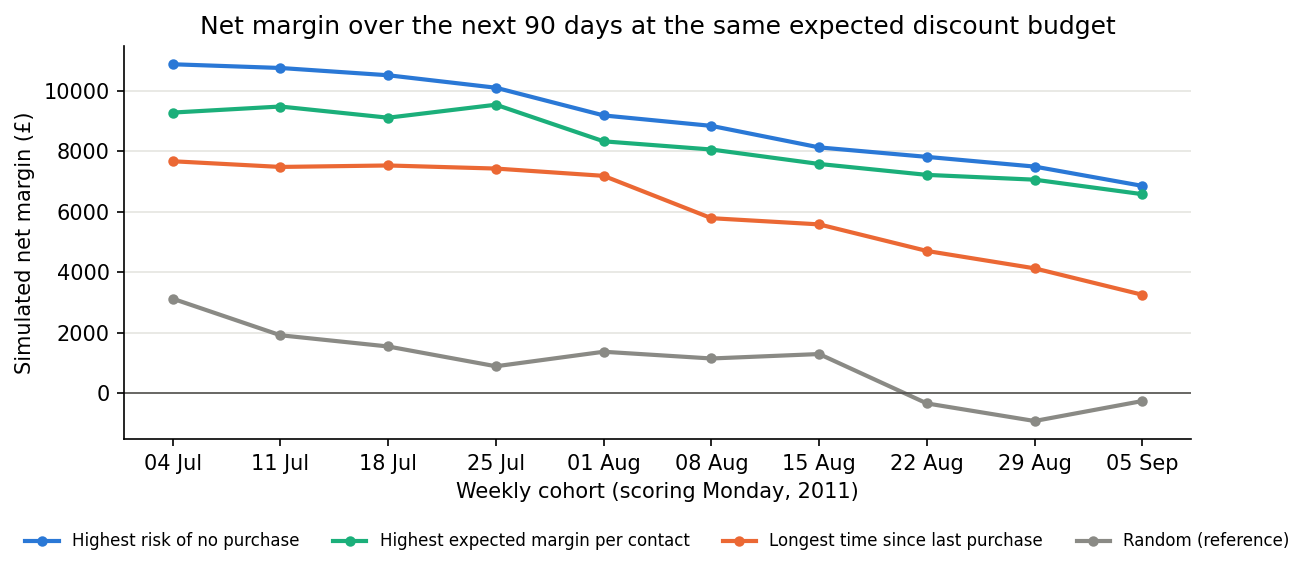
\includegraphics[width=0.9\textwidth]{figures/ch7_equal_budget_weekly.png}
\end{center}

Four observations:
\begin{enumerate}
    \item \textbf{The model creates the value.} With the same expected discount spend, ranking by churn risk adds \textbf{\pounds2,982 (49\%)} more simulated margin than the longest-inactive rule and leads it \textbf{in all ten test weeks}. It reaches 521 would-be churners per week against 378 for the recency rule, so more of the budget goes to customers whose purchase can be recovered: \pounds1.10 of margin per \pounds1 of expected discount (\pounds1.08 per \pounds1 of discount actually given).
    \item \textbf{Adding customer value does not raise the total at equal spend.} The expected-margin list favors customers with large orders, whose vouchers cost more, so the same budget reaches only 485 customers. It earns \pounds833 less than the risk-ranked list and trails it in all ten weeks, but uses 341 fewer contacts: it is the lighter option when contact capacity, not the discount budget, is the binding constraint (Section~\ref{sec:8-3}).
    \item \textbf{Untargeted offers waste the budget.} A random list of the same cost earns \pounds979 and turns negative in the last three weeks: most of its vouchers go to customers who would have bought anyway.
    \item \textbf{The level moves with the season, the order does not.} Every list earns less from July to September because later cohorts' 90-day windows run into the pre-Christmas season, when fewer customers churn (Section~\ref{sec:5-4}); the ranking of the lists is the same in every week.
\end{enumerate}

\textbf{Ranking quality.} On the same test rows, the calibrated churn probability reaches an AUC of 0.759, against 0.638 for days since the last purchase and 0.496 for random -- the predictive criterion of Section~\ref{sec:2-6}. The targeting and business-scenario criteria are met as well: the model-ranked list reaches more would-be churners than the recency rule at the same spend, and its simulated margin is positive and higher in all ten weeks.

\textbf{The discount given differs slightly from the plan.} Each list spends about 1--2\% more than expected (\pounds8,357 against \pounds8,213 for the risk-ranked list). The expected cost uses the calibrated probability, which overestimates churn slightly in the test weeks (0.418 against 0.401); since would-be buyers redeem more often than would-be churners ($r > e$), overestimating churn underestimates the cost. Recalibrating on recent weeks (Section~\ref{sec:8-7}) keeps the spend on budget.

\section{Scenario Analysis}
\label{sec:7-5}

\textbf{Voucher depth.} Three offers, each with its own budget recomputed from that scenario's expected-margin list:

\begin{center}
\footnotesize
\setlength{\tabcolsep}{4pt}
\begin{tabular}{@{}p{1.6cm}rrrrrrr@{}}
    \toprule
    Scenario & \shortstack[r]{Voucher\\$d$} & \shortstack[r]{Response\\$e$} & \shortstack[r]{Weekly\\budget} & \shortstack[r]{Risk-ranked\\contacts} & \shortstack[r]{Highest\\risk} & \shortstack[r]{Expected-\\margin list} & \shortstack[r]{Longest since\\purchase} \\
    \midrule
    Light & 5\% & 20\% & \pounds3,725 & 906 & \textbf{\pounds8,754} & \pounds7,766 & \pounds6,224 \\
    \textbf{Base} & 10\% & 30\% & \pounds8,219 & 826 & \textbf{\pounds9,060} & \pounds8,228 & \pounds6,079 \\
    Deep & 20\% & 40\% & \pounds14,866 & 664 & \textbf{\pounds3,695} & \pounds3,173 & \pounds664 \\
    \bottomrule
\end{tabular}
\end{center}

Ranking by churn risk earns the most in every scenario and leads the longest-inactive rule in all ten weeks of each; it leads the expected-margin list in 10, 10 and 9 of the ten weeks. A deeper voucher brings back more customers but gives away twice the discount on every redeemed order, so a 20\% voucher earns far less than a 10\% one despite a budget almost twice as large. The 10\% Base scenario is the starting point for the pilot (Chapter~\ref{ch:conclusion}).

\textbf{Gross margin.} The data hold revenue only, so $m$ is an assumption; Base voucher, each margin at its own equal budget:

\begin{center}
\footnotesize
\begin{tabular}{@{}p{2.2cm}rrrrr@{}}
    \toprule
    Gross margin $m$ & \shortstack[r]{Weekly\\budget} & \shortstack[r]{Risk-ranked\\contacts} & \shortstack[r]{Highest\\risk} & \shortstack[r]{Expected-\\margin list} & \shortstack[r]{Longest since\\purchase} \\
    \midrule
    30\% & \pounds7,294 & 755 & \textbf{\pounds4,369} & \pounds3,989 & \pounds2,291 \\
    \textbf{40\%} & \pounds8,219 & 826 & \textbf{\pounds9,060} & \pounds8,228 & \pounds6,079 \\
    50\% & \pounds8,744 & 867 & \textbf{\pounds14,132} & \pounds12,670 & \pounds10,103 \\
    \bottomrule
\end{tabular}
\end{center}

The order of the three lists does not change with the margin, but the level does: at a 30\% margin a \pounds300 order won back contributes only \pounds60 after the voucher, and the risk-ranked list earns less than half of its Base margin. Finance should confirm actual product margins before launch.

\section{Error Analysis and Limitations}
\label{sec:7-12}

As a fixed diagnostic of the model's ranking (\texttt{notebooks/05\_scoring.ipynb}), the top 10\% of the test rows by the final model's score are treated as ``targeted'' and the errors are broken down by segment (one-time vs repeat), country (UK vs non-UK) and wholesale-sized customers. Pooled across the test period: 57.5\% true negatives, 32.5\% false negatives, 7.6\% true positives, 2.4\% false positives -- the false-negative share is large by construction, since a 10\%-wide net cannot catch most of a $\approx$40\% base rate.

\begin{center}
\begin{tabular}{@{}p{3.6cm}p{2.6cm}p{2.6cm}@{}}
    \toprule
    Group & FP rate (among targeted) & FN rate (among non-targeted) \\
    \midrule
    One-time & 23.6\% & 54.8\% \\
    Repeat & 25.7\% & 34.6\% \\
    \midrule
    UK & 23.4\% & 36.5\% \\
    Non-UK & 36.7\% & 32.5\% \\
    \midrule
    Retail & 24.3\% & 37.0\% \\
    Wholesale-like & n/a (0 targeted) & 5.6\% \\
    \bottomrule
\end{tabular}
\end{center}

Three patterns stand out. \textbf{One-time customers} are missed far more often than repeat customers (54.8\% vs.\ 34.6\% FN rate) -- with only one purchase occasion, their feature history is thin, and the model has less signal to work with (the one-time group of Section~\ref{sec:4-4}); the pilot therefore reports one-time and repeat buyers separately (Chapter~\ref{ch:conclusion}). \textbf{Non-UK customers} see a clearly higher false-positive rate (36.7\% vs.\ 23.4\% for UK) -- the model, trained overwhelmingly on UK behavior (Section~\ref{sec:4-2}), generalizes less cleanly to the small non-UK population (9.6\% of test rows). \textbf{Wholesale-like customers} (monetary value so far at or above the train period's 99th percentile; 658 test rows) are the model's strongest case: a 5.6\% false-negative rate, far below retail's 37.0\%, and none were false positives in the targeted top 10\% -- their high, frequent purchase volume makes their churn signal unusually clear.

\textbf{Limitations of the simulation.} Online Retail II contains no campaign treatment/control information, so the response $e$, the redemption $r$ and the margin $m$ are assumptions, and incremental revenue, causal retention effect and true campaign ROI cannot be identified from this data. The results cover a single test season (Jul--Sep 2011), and the weekly cohorts overlap. Chapter~\ref{ch:robustness} discusses how far the conclusions depend on these choices.

\textbf{Principle.} The model identifies and prioritizes churn risk; the retention campaign determines treatment; actual incremental profit requires treatment/control data. Every margin figure in this chapter is a simulation output until a pilot with a no-offer control group measures it (Chapter~\ref{ch:conclusion}).
